\documentclass[11pt,a4paper]{article}

% ---- Packages ----
\usepackage[utf8]{inputenc}
\usepackage[T1]{fontenc}
\usepackage[english]{babel}

\usepackage[margin=1.1in]{geometry}
\usepackage{amsmath, amssymb, amsthm, mathtools}
\usepackage{booktabs, array}
\usepackage{enumitem}
\usepackage{xcolor}
\usepackage{graphicx}
\usepackage{epigraph}
\usepackage{csquotes}
\usepackage{tikz}
\usetikzlibrary{arrows.meta, positioning, shapes.geometric, shapes.misc,
                fit, calc, backgrounds, decorations.pathreplacing,
                patterns, matrix}
\usepackage{pgfplots}
\pgfplotsset{compat=1.18}

\usepackage[colorlinks=true, linkcolor=black!70!blue,
            citecolor=black!70!blue, urlcolor=black!40!blue]{hyperref}

% ---- Theorem environments ----
\theoremstyle{definition}
\newtheorem{definition}{Definition}[section]
\newtheorem{example}[definition]{Example}

\theoremstyle{remark}
\newtheorem*{remark}{Remark}
\newtheorem*{aside}{Aside}

\theoremstyle{plain}
\newtheorem{proposition}[definition]{Proposition}

% ---- Epigraph style ----
\setlength{\epigraphwidth}{0.6\textwidth}
\renewcommand{\epigraphflush}{flushright}
\renewcommand{\textflush}{flushright}
\renewcommand{\epigraphsize}{\small\itshape}

% ---- Small conveniences ----
\newcommand{\todo}[1]{\textcolor{red!70!black}{\textbf{[TODO: #1]}}}
\newcommand{\ai}{\text{AI}}
\newcommand{\flop}{\mathrm{FLOP}}
\newcommand{\flops}{\mathrm{FLOPs}}
\DeclareMathOperator*{\argmin}{arg\,min}

% ---- Title ----
\title{\textbf{Efficient Deep Learning Systems} \\[0.3em]
       \large Lecture 1 --- Course Introduction, GPU Computing, \\
       and the Roofline Model}
\author{Lecture notes}
\date{}

\begin{document}
\sloppy
\maketitle


\begin{abstract}
\noindent
These notes accompany the opening lecture of a course on efficient
deep learning systems. We motivate the study of systems engineering
for large-scale machine learning, survey the logistics of
the course, and then descend from the bird's-eye view into the
hardware that makes modern deep learning possible. Along the way we
meet the GPU, the SIMT execution model, the CUDA programming
abstraction, the memory hierarchy, tile and wave quantisation, and
finally the Roofline model --- the lingua franca for reasoning about
whether a computation is limited by arithmetic or by memory.
\end{abstract}

\tableofcontents
\bigskip
\hrule
\bigskip

%%%%%%%%%%%%%%%%%%%%%%%%%%%%%%%%%%%%%%%%%%%%%%%%%%%%%%%%%%%%%%%%%%%%%%%%
\section{Why Are We Here?}
%%%%%%%%%%%%%%%%%%%%%%%%%%%%%%%%%%%%%%%%%%%%%%%%%%%%%%%%%%%%%%%%%%%%%%%%

Deep learning has entered a phase of \emph{maturity}. Neural networks
have migrated from the blackboards of academic labs into the machinery
of industry, where they now power products used by hundreds of
millions of people. This transition is not merely sociological; it has
consequences for how we build and reason about the systems that train
and serve these models.

Three scaling trends define the contemporary landscape. First, models
have grown: frontier systems now comprise tens or hundreds of billions
of parameters, and in some cases more. Second, datasets have grown
with them, from the megabytes of early benchmarks to the petabytes of
today's pre-training corpora. Third, the collaborations themselves
have grown, visible in the ever-lengthening author lists of the
papers that push the field forward.

These trends have rendered the traditional development paradigm ---
the single-researcher, single-notebook workflow rooted in
\texttt{.ipynb} files --- largely inadequate at the frontier. The
Jupyter notebook remains a superb instrument for prototyping and
exploration, but it is not a vehicle for managing thousand-GPU
training runs, enforcing reproducibility across months of
experimentation, or orchestrating the release pipelines of a
production model. To do any of these things seriously one must adopt
the tools and discipline of software engineering.

\begin{remark}
A useful heuristic: if one cannot plausibly claim that a proposed
technique would survive contact with a realistic training and
deployment regime, the proposal remains theoretical. State-of-the-art
research is increasingly gated not by architectural imagination alone
but by the engineering proficiency to execute on it.
\end{remark}

%%%%%%%%%%%%%%%%%%%%%%%%%%%%%%%%%%%%%%%%%%%%%%%%%%%%%%%%%%%%%%%%%%%%%%%%
\section{A Bird's-Eye View of the Deep Learning Lifecycle}
%%%%%%%%%%%%%%%%%%%%%%%%%%%%%%%%%%%%%%%%%%%%%%%%%%%%%%%%%%%%%%%%%%%%%%%%

At the highest level of abstraction, the life of a deep learning model
consists of two phases, each governed by its own set of concerns.

\begin{center}
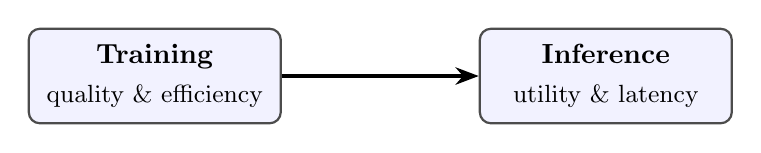
\begin{tikzpicture}[
    phase/.style={rectangle, rounded corners, draw=black!70, thick,
                  fill=blue!5, minimum width=3.2cm, minimum height=1.2cm,
                  align=center},
    arr/.style={-Stealth, very thick}
]
\node[phase] (tr) {\textbf{Training}\\[2pt]\small quality \& efficiency};
\node[phase, right=2.5cm of tr] (inf) {\textbf{Inference}\\[2pt]\small utility \& latency};
\draw[arr] (tr) -- (inf);
\end{tikzpicture}
\end{center}

\subsection{The Training Phase}

During training the central concern is \emph{quality}: how do we
produce the best possible model for the task (or, in the case of
foundation models, across a broad distribution of tasks)?
Operationally, this decomposes into four intertwined questions:

\begin{itemize}[leftmargin=1.5em, itemsep=2pt]
    \item \textbf{Model quality.} What architectural, optimisation,
          and data choices maximise task performance?
    \item \textbf{Experimental velocity.} How fast can we iterate? A
          day saved per experiment compounds across the lifetime of a
          project.
    \item \textbf{Hardware utilisation.} Are we using the GPUs and
          TPUs we have paid for? An under-utilised accelerator is the
          most expensive idle thing in a data centre.
    \item \textbf{Infrastructure planning.} How much compute, memory,
          and interconnect will a run of a given scale consume, and
          when?
\end{itemize}

A persistent hazard of the training phase is the deceptive nature of
benchmark metrics. A model that attains high accuracy on a chosen
evaluation set may fail catastrophically under a distribution shift
--- for example, a classifier trained on literary prose confronted
with spoken dialogue. Designing an honest experimental protocol is
therefore part of the scientific method, not an afterthought.

\subsection{The Inference Phase}

At inference time the question changes from \emph{how good?} to
\emph{is it good enough, fast enough, and cheap enough?} The
considerations become:

\begin{itemize}[leftmargin=1.5em, itemsep=2pt]
    \item \textbf{Utility.} Does the model solve the actual problem
          the user has?
    \item \textbf{Accuracy under deployment conditions.} Accuracy in
          the wild, not on the held-out test set.
    \item \textbf{Latency and throughput.} A model that takes thirty
          seconds to respond is unusable in a chat interface and
          ruinous in a high-throughput pipeline.
    \item \textbf{Scalability.} A demonstration serves ten users; a
          launch serves hundreds of thousands. The transition is
          rarely graceful.
    \item \textbf{Cost.} If the cost of a single query exceeds the
          revenue it generates, the business does not survive contact
          with its users.
    \item \textbf{Safety.} The ethical and societal implications of
          large generative systems constitute an active area of
          research and governance.
\end{itemize}

\begin{remark}
The two phases are not independent. Decisions made during training
---quantisation-awareness, architectural choices, the batch dimension
of attention --- propagate directly into the economics of inference.
A systems-minded practitioner treats the lifecycle holistically.
\end{remark}

%%%%%%%%%%%%%%%%%%%%%%%%%%%%%%%%%%%%%%%%%%%%%%%%%%%%%%%%%%%%%%%%%%%%%%%%
\section{Course Structure and Logistics}
%%%%%%%%%%%%%%%%%%%%%%%%%%%%%%%%%%%%%%%%%%%%%%%%%%%%%%%%%%%%%%%%%%%%%%%%

\subsection{Scope and Pedagogical Stance}

Knowledge about efficient deep learning is scattered across blog
posts, conference papers, framework documentation, and lecture videos
of wildly varying quality. The aim of this course is to offer a
\emph{curated} and \emph{structured} reference, biased toward
techniques that have proved themselves stable over time rather than
the transient fashions of the last preprint cycle. Six pillars guide
our selection of material:

\begin{enumerate}[leftmargin=1.8em, itemsep=2pt]
    \item Practical application over pure theory.
    \item Computational efficiency --- the surprising power of small
          code changes.
    \item Deployment and scalability, both as standalone systems and
          as components of larger architectures.
    \item Maintenance: treating ML models as proper software
          artefacts subject to testing, versioning, and operational
          hygiene.
    \item Curated knowledge in place of doomscrolling arXiv.
    \item An applied focus that privileges methods which have earned
          a place in industry practice.
\end{enumerate}

\subsection{Structure}

The course runs for nine weeks. After this introductory week, a
substantial block is devoted to large-scale training: three lectures
on distributed training and a detailed treatment of the arithmetic
and performance characteristics of the training process. A final
block of three specialised sessions concludes the term, covering
topics such as open-source ML-system repositories and a spectrum of
testing methodologies from the lightweight to the computationally
extravagant.

Lectures and seminars meet on Wednesdays, either in person or via
Zoom, with the mode of instruction announced in advance. Course
materials and assignments live in the public course repository,
\href{https://github.com/mryab/efficient-dl-systems}{\texttt{github.com/mryab/efficient-dl-systems}}.

\bigskip\hrule\bigskip

%%%%%%%%%%%%%%%%%%%%%%%%%%%%%%%%%%%%%%%%%%%%%%%%%%%%%%%%%%%%%%%%%%%%%%%%
\section{The Rise of the GPU}
%%%%%%%%%%%%%%%%%%%%%%%%%%%%%%%%%%%%%%%%%%%%%%%%%%%%%%%%%%%%%%%%%%%%%%%%

To understand why deep learning looks the way it does, one must
understand the hardware upon which it is run. Almost every neural
network --- even the simplest feed-forward one --- spends the
overwhelming majority of its computational budget inside a few
matrix multiplications (GEMMs), interleaved with comparatively
lightweight element-wise operations and normalisations.
Matrix multiplication is \emph{embarrassingly parallel}, and in the
late 2000s the hardware community finally possessed a device with an
embarrassment of parallel arithmetic units ready to exploit it: the
graphics processing unit.

\subsection{From Voodoo to Blackwell: a Short History}

The GPU was born for graphics. The \textit{3dfx Voodoo2} of the late
1990s, with its meagre 12\,MB of RAM, existed to rasterise triangles
for video games. Rendering a scene, however, turns out to require
millions of broadly independent linear-algebraic operations per
frame --- a workload uncannily similar to the one a neural network
demands.

Around 2007 this latent generality was unlocked by general-purpose
GPU (GPGPU) programming interfaces: NVIDIA's CUDA, the open OpenCL
standard. In the early 2010s, AlexNet and its
contemporaries demonstrated that training large convolutional
networks on GPUs crossed a threshold of practicality that had
eluded CPU-only attempts, inaugurating what is now sometimes called
the deep learning revolution.

Modern data-centre accelerators such as the NVIDIA GB200 NVL72 now
carry hundreds of gigabytes of memory, require liquid cooling, and
draw the power of a small village --- a trajectory that raises
legitimate environmental questions. The gains in capability,
however, are measured in orders of magnitude.

\subsection{CPU versus GPU: Divergent Design Philosophies}

Both CPUs and GPUs organise memory hierarchically, and both execute
instructions fetched from that memory. They differ in what they
optimise for.

A CPU is a \emph{latency-optimised} machine. It possesses a small
number of powerful cores, deep caches (L1, L2, L3), sophisticated
branch prediction, and elaborate control logic, all aimed at making
a single stream of instructions finish as quickly as possible.

A GPU is a \emph{throughput-optimised} machine. It sacrifices
per-thread latency for the ability to keep thousands of arithmetic
lanes busy simultaneously. Its control logic is comparatively
simple, its caches are smaller relative to its compute, and it wins
by the sheer quantity of work completed per unit time.

\begin{center}
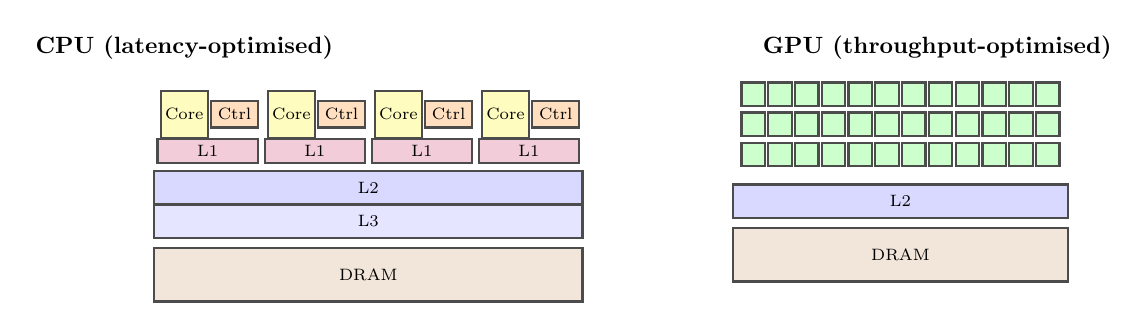
\begin{tikzpicture}[scale=0.85, transform shape,
    box/.style={rectangle, draw=black!70, thick, minimum width=0.8cm,
                minimum height=0.5cm, inner sep=1pt, font=\scriptsize},
    label/.style={font=\small\bfseries},
    title/.style={font=\bfseries}
]
% -------- CPU --------
\node[title] at (0, 5.2) {CPU (latency-optimised)};

% Four fat cores with control and L1
\foreach \x in {0,1.6,3.2,4.8} {
    \node[box, fill=yellow!25, minimum width=0.7cm, minimum height=0.7cm]
        at (\x, 4.2) {Core};
    \node[box, fill=orange!25, minimum width=0.7cm, minimum height=0.4cm]
        at (\x+0.75, 4.2) {Ctrl};
    \node[box, fill=purple!20, minimum width=1.5cm, minimum height=0.35cm]
        at (\x+0.35, 3.65) {L1};
}
\node[box, fill=blue!15, minimum width=6.4cm] at (2.75, 3.1) {L2};
\node[box, fill=blue!10, minimum width=6.4cm] at (2.75, 2.6) {L3};
\node[box, fill=brown!20, minimum width=6.4cm, minimum height=0.8cm]
    at (2.75, 1.8) {DRAM};

% -------- GPU --------
\begin{scope}[xshift=8.5cm]
\node[title] at (2.75, 5.2) {GPU (throughput-optimised)};
% Dense grid of small cores
\foreach \i in {0,...,11} {
    \foreach \j in {0,1,2} {
        \node[box, fill=green!20, minimum width=0.35cm,
              minimum height=0.35cm, inner sep=0.3pt] at
              (0.4*\i, 4.5 - 0.45*\j) {};
    }
}
\node[box, fill=blue!15, minimum width=5cm] at (2.2, 2.9) {L2};
\node[box, fill=brown!20, minimum width=5cm, minimum height=0.8cm]
    at (2.2, 2.1) {DRAM};
\end{scope}
\end{tikzpicture}
\end{center}

The geometry is instructive: the CPU devotes most of its silicon to
\emph{control}, the GPU to \emph{arithmetic}. These are two
fundamentally different bets about what the machine will spend its
time doing. (The comparison originates in NVIDIA's \textit{CUDA C
Programming Guide}.\footnote{\url{https://docs.nvidia.com/cuda/cuda-c-programming-guide}})

%%%%%%%%%%%%%%%%%%%%%%%%%%%%%%%%%%%%%%%%%%%%%%%%%%%%%%%%%%%%%%%%%%%%%%%%
\section{The CUDA Computation Model}
%%%%%%%%%%%%%%%%%%%%%%%%%%%%%%%%%%%%%%%%%%%%%%%%%%%%%%%%%%%%%%%%%%%%%%%%

\subsection{Host, Device, and Kernels}

The CUDA model distinguishes a \emph{host} (the CPU) from a
\emph{device} (the GPU). A program written for the device is called
a \emph{kernel}. The host is responsible for preparing data,
launching kernels, and collecting results; the device executes each
kernel in parallel across a large number of lightweight threads.

\begin{definition}[Kernel]
A kernel is a function, written in CUDA C/C++ (or emitted by a
higher-level compiler such as Triton), whose body is executed
concurrently by many GPU threads. Each thread receives an index,
typically accessed through built-in variables such as
\texttt{threadIdx}, \texttt{blockIdx}, and \texttt{blockDim}, which
it uses to decide what slice of the input to process.
\end{definition}

\subsection{The Execution Hierarchy}

Threads are not loose particles; they inhabit a three-level
hierarchy whose logical structure is mirrored in the physical
hardware.

\begin{center}
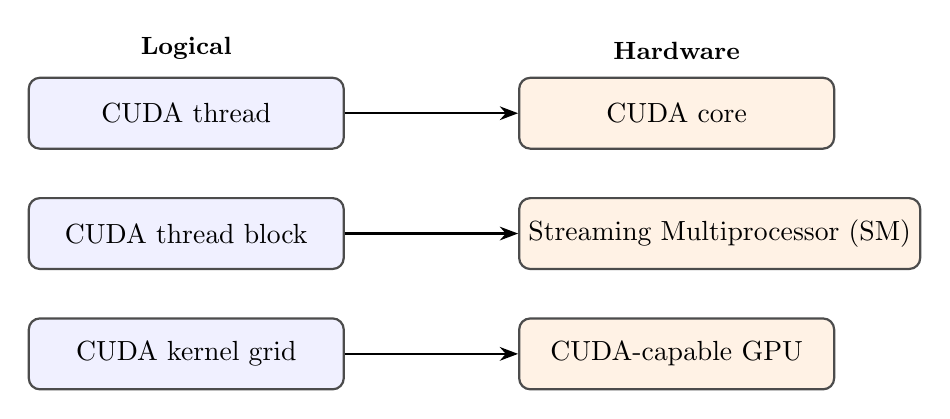
\begin{tikzpicture}[
    node distance=0.6cm,
    box/.style={rectangle, rounded corners, draw=black!70, thick,
                fill=blue!6, minimum width=4cm, minimum height=0.9cm,
                align=center},
    hw/.style  ={rectangle, rounded corners, draw=black!70, thick,
                fill=orange!10, minimum width=4cm, minimum height=0.9cm,
                align=center},
    arr/.style={-Stealth, thick}
]
\node[box] (th)  {CUDA thread};
\node[box, below=of th] (tb)  {CUDA thread block};
\node[box, below=of tb] (gr)  {CUDA kernel grid};

\node[hw, right=2.2cm of th] (co)  {CUDA core};
\node[hw, right=2.2cm of tb] (sm)  {Streaming Multiprocessor (SM)};
\node[hw, right=2.2cm of gr] (gpu) {CUDA-capable GPU};

\draw[arr] (th) -- (co);
\draw[arr] (tb) -- (sm);
\draw[arr] (gr) -- (gpu);

\node[above=0.1cm of th, font=\small\bfseries] {Logical};
\node[above=0.1cm of co, font=\small\bfseries] {Hardware};
\end{tikzpicture}
\end{center}

A \emph{thread} is the smallest unit of work and is executed by a
single CUDA core. Threads are grouped into \emph{thread blocks} of
bounded size; a block is the smallest unit of cooperation and is
always scheduled onto a single Streaming Multiprocessor (SM), which
allows the threads within it to share fast on-chip memory and to
synchronise. The collection of all blocks launched by a single
kernel call constitutes the \emph{grid}, which may be organised in
one, two, or three logical dimensions and which, as a whole, is the
work the GPU has been asked to do. (This mapping follows NVIDIA's
\href{https://developer.nvidia.com/blog/cuda-refresher-cuda-programming-model/}{\textit{CUDA
Refresher: The CUDA Programming Model}}.)

\begin{remark}
One sometimes asks: why not simply launch a million threads and
execute them simultaneously? The answer is hardware. A GPU has a
finite number of SMs, each with a finite number of lanes. The
hierarchy is not decorative; it is how the runtime maps an
arbitrarily large logical workload onto a physically bounded
machine.
\end{remark}

\subsection{SIMT and the Warp}

On the hardware, threads are not in fact individuals. They travel in
groups of thirty-two, called \emph{warps}, and all threads in a
warp execute the same instruction in the same cycle. This is the
\textbf{SIMT} (Single Instruction, Multiple Thread) model that
NVIDIA hardware implements.

\begin{definition}[Warp]
A warp is a group of $32$ threads scheduled and executed as a
single SIMD-like unit by an SM. Warps are the atoms of GPU
scheduling.
\end{definition}

The consequence for the programmer is subtle and important. Consider
an \texttt{if/else} in a kernel:

\begin{quote}\small
\texttt{if (cond) \{ A(); \} else \{ B(); \}}
\end{quote}

If all threads in a warp agree on \texttt{cond}, exactly one branch
executes and the other is skipped. If they disagree --- a situation
known as \emph{warp divergence} --- the hardware executes both
branches sequentially, masking off the threads that do not belong to
the path currently in flight. The answer remains mathematically
correct, but half the lanes sit idle for half the time. In
pathological cases (e.g.\ $n$-way divergence) one can lose a factor
of $n$ in throughput.

\begin{remark}[Warp-level primitives]
Recent CUDA generations expose instructions such as
\texttt{\_\_shfl\_down\_sync}, \texttt{\_\_shfl\_xor\_sync}, and
\texttt{\_\_ballot\_sync}, which allow threads within a warp to
exchange data directly through register-to-register shuffles, without
going through shared memory. Used carefully, these primitives can
collapse reductions and scans into a handful of instructions. A
canonical reduction fragment:
\begin{quote}\small
\texttt{v += \_\_shfl\_down\_sync(mask, v, 16);} \\
\texttt{v += \_\_shfl\_down\_sync(mask, v, \phantom{1}8);} \\
\texttt{v += \_\_shfl\_down\_sync(mask, v, \phantom{1}4);} \\
\texttt{v += \_\_shfl\_down\_sync(mask, v, \phantom{1}2);} \\
\texttt{v += \_\_shfl\_down\_sync(mask, v, \phantom{1}1);}
\end{quote}
reduces a warp of $32$ values to a single sum in five rounds. NVIDIA's
\href{https://developer.nvidia.com/blog/using-cuda-warp-level-primitives/}{\textit{Using
CUDA Warp-Level Primitives}} walks through these in detail.
\end{remark}

For a more thorough treatment the reader is referred to the
\textit{CUDA C Programming Guide},
\url{https://docs.nvidia.com/cuda/cuda-c-programming-guide/}.

%%%%%%%%%%%%%%%%%%%%%%%%%%%%%%%%%%%%%%%%%%%%%%%%%%%%%%%%%%%%%%%%%%%%%%%%
\section{Tile and Wave Quantisation}
%%%%%%%%%%%%%%%%%%%%%%%%%%%%%%%%%%%%%%%%%%%%%%%%%%%%%%%%%%%%%%%%%%%%%%%%

Having described the abstract machine, we can now see why
apparently innocuous choices --- an embedding dimension of $257$
instead of $256$, say --- can wreck throughput. The culprits are
two related phenomena known as \emph{tile quantisation} and
\emph{wave quantisation}. The examples and measurements in this
section come from NVIDIA's deep learning performance documentation on
matrix multiplication.\footnote{%
\url{https://docs.nvidia.com/deeplearning/performance/dl-performance-matrix-multiplication/index.html}}

\subsection{Tile Quantisation}

A large GEMM, say $C = A B$ with $A \in \mathbb{R}^{M \times K}$ and
$B \in \mathbb{R}^{K \times N}$, cannot be computed by a single
thread block; there simply isn't enough register file or shared
memory. Instead, the output $C$ is decomposed into two-dimensional
\emph{tiles} of some fixed size (for instance $128 \times 128$), each
of which is assigned to one thread block.

\begin{definition}[Tile quantisation]
Tile quantisation is the phenomenon whereby the output dimensions of
a GEMM are not integer multiples of the chosen tile dimensions. The
excess boundary is nonetheless processed by a full tile --- the
hardware cannot spawn a fractional thread block --- leading to
underutilised lanes inside those edge tiles.
\end{definition}

An analogy. Suppose one is baking cookies on trays of twenty, and one
needs to bake twenty-one cookies. One tray holds twenty; the
twenty-first cookie commandeers an entire second tray on its own.
The oven is nineteen-twentieths empty during that second bake. A GPU
executing a GEMM whose dimensions are $256 \times 257$ faces exactly
this situation: a thick band of fully utilised tiles, and a thin
column of nearly empty ones.

\subsection{Wave Quantisation}

The second effect concerns the scheduling of tiles onto SMs. The
GPU launches tiles in \emph{waves}: at any given moment, each SM is
working on one (or a small, fixed number of) tile, and a wave is the
set of tiles in flight together.

\begin{definition}[Wave quantisation]
Wave quantisation is the phenomenon whereby the total number of
tiles in a computation is not an integer multiple of the number of
SMs. The final, partially-populated wave --- the \emph{tail wave}
--- leaves some SMs idle, and this idleness is pure waste.
\end{definition}

\begin{center}
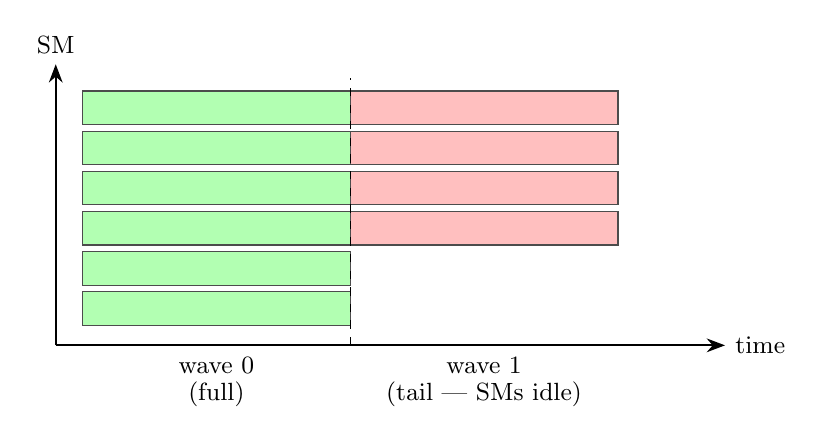
\begin{tikzpicture}[scale=0.85,
    axlabel/.style={font=\small}]
\draw[-Stealth, thick] (0,0) -- (10,0) node[right] {\small time};
\draw[-Stealth, thick] (0,0) -- (0,4.2) node[above] {\small SM};

% Wave 0 - full
\foreach \y in {0.3, 0.9, 1.5, 2.1, 2.7, 3.3} {
    \fill[green!30, draw=black!70] (0.4, \y) rectangle (4.4, \y+0.5);
}
\node[align=center] at (2.4, -0.55) {\small wave 0 \\[-2pt]\small (full)};

% Wave 1 - tail
\foreach \y in {1.5, 2.1, 2.7, 3.3} {
    \fill[red!25, draw=black!70] (4.4, \y) rectangle (8.4, \y+0.5);
}
\node[align=center] at (6.4, -0.55) {\small wave 1 \\[-2pt]\small (tail --- SMs idle)};

\draw[dashed] (4.4, 0) -- (4.4, 4);
\end{tikzpicture}
\end{center}

Empirically, one observes that throughput as a function of a matrix
dimension $N$ is not smooth but \emph{staircase-like}: plateaus of
constant throughput, punctuated by sudden drops as one crosses a
tile or wave boundary. Duration behaves inversely. The moral: when
dimensioning hidden layers, attention heads, or batch sizes, a small
amount of arithmetic with respect to the tile and wave sizes of the
target hardware can yield outsized performance dividends.

%%%%%%%%%%%%%%%%%%%%%%%%%%%%%%%%%%%%%%%%%%%%%%%%%%%%%%%%%%%%%%%%%%%%%%%%
\section{The Memory Hierarchy and the Data Transfer Bottleneck}
%%%%%%%%%%%%%%%%%%%%%%%%%%%%%%%%%%%%%%%%%%%%%%%%%%%%%%%%%%%%%%%%%%%%%%%%

A GPU is, above all, a memory system with some arithmetic attached.
Understanding the layers of that memory system --- and the cost of
moving bytes between them --- is therefore the most important
performance discipline we will develop.

\subsection{Host--Device Transfers}

GPU memory (sometimes called \emph{device memory} or VRAM) is
physically and logically distinct from host memory. Data must be
explicitly copied across the PCIe bus; for PCIe~4.0~$\times 16$ the
peak bandwidth is roughly $32\,\text{GB/s}$, a figure that is
laughably small next to the internal bandwidth of a modern GPU's
HBM. Host--device transfer is, accordingly, a frequent bottleneck.
(The pageable-versus-pinned comparison below is taken from NVIDIA's
\href{https://developer.nvidia.com/blog/how-optimize-data-transfers-cuda-cc/}{\textit{How
to Optimize Data Transfers in CUDA C/C++}}.)

One distinguishes two kinds of transfer:

\begin{description}[leftmargin=1.8em, style=nextline]
    \item[Pageable transfer.] The host buffer lives in ordinary,
        pageable virtual memory. The operating system is free to
        swap its pages, so before a transfer the driver must first
        copy the data into a temporary pinned staging buffer, and
        only then may DMA(Direct Memory Access) commence. Two copies, one slow.
    \item[Pinned (page-locked) transfer.] The host buffer has been
        marked as page-locked, so the OS is forbidden from swapping
        it. The GPU's DMA engine can read it directly. One copy,
        fast and predictable.
\end{description}

\begin{center}
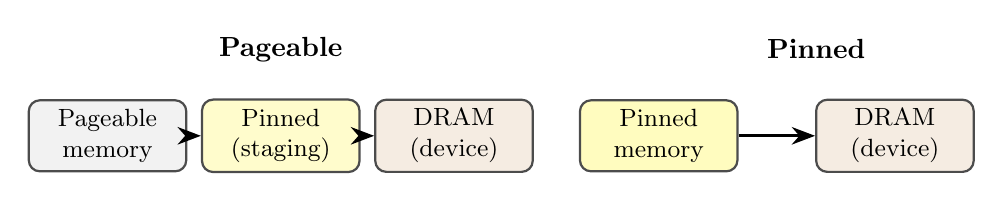
\begin{tikzpicture}[
    box/.style={rectangle, rounded corners, draw=black!70, thick,
                minimum width=2.0cm, minimum height=0.8cm,
                align=center, font=\small},
    arr/.style={-Stealth, very thick}
]
% Pageable
\node[font=\bfseries] at (2.2, 3.3) {Pageable};
\node[box, fill=gray!10]   (pa) at (0,   2.2) {Pageable\\memory};
\node[box, fill=yellow!20] (ps) at (2.2, 2.2) {Pinned\\(staging)};
\node[box, fill=brown!15]  (pd) at (4.4, 2.2) {DRAM\\(device)};
\draw[arr] (pa) -- (ps);
\draw[arr] (ps) -- (pd);

% Pinned
\node[font=\bfseries] at (9.0, 3.3) {Pinned};
\node[box, fill=yellow!25] (np) at (7.0, 2.2) {Pinned\\memory};
\node[box, fill=brown!15]  (nd) at (10.0, 2.2) {DRAM\\(device)};
\draw[arr] (np) -- (nd);
\end{tikzpicture}
\end{center}

The empirical difference is substantial. Plotting transfer time
versus data size reveals that pageable transfers grow with a
significantly steeper slope than pinned transfers; at a few hundred
megabytes the gap is easily a factor of two or more. Pinned memory
is not free --- it is a finite physical resource and cannot be used
indiscriminately --- but for training pipelines that stream large
tensors to the device, it is indispensable.

\subsection{The On-Device Hierarchy}

On the device itself, the programmer is presented with a hierarchy
that trades capacity for speed:

\begin{center}
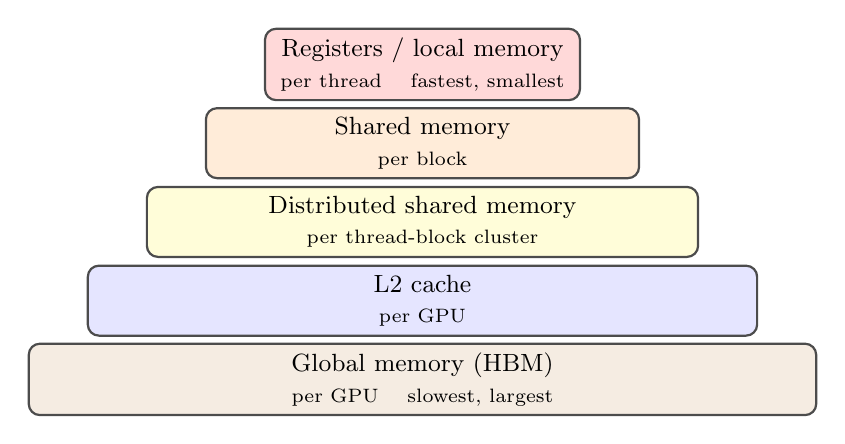
\begin{tikzpicture}[
    lvl/.style={rectangle, rounded corners, draw=black!70, thick,
                align=center, font=\small,
                minimum height=0.7cm},
    arr/.style={-Stealth, thick}
]
\node[lvl, fill=red!15,    minimum width=4.0cm] (r)   at (0, 4.0) {Registers / local memory \\ \scriptsize per thread \hspace{5pt} fastest, smallest};
\node[lvl, fill=orange!15, minimum width=5.5cm] (s)   at (0, 3.0) {Shared memory \\ \scriptsize per block};
\node[lvl, fill=yellow!15, minimum width=7.0cm] (c)   at (0, 2.0) {Distributed shared memory \\ \scriptsize per thread-block cluster};
\node[lvl, fill=blue!10,   minimum width=8.5cm] (l2)  at (0, 1.0) {L2 cache \\ \scriptsize per GPU};
\node[lvl, fill=brown!15,  minimum width=10cm]  (gm)  at (0, 0.0) {Global memory (HBM) \\ \scriptsize per GPU \hspace{5pt} slowest, largest};
\end{tikzpicture}
\end{center}

Registers are private to a thread and give sub-nanosecond access.
Shared memory is an on-chip scratchpad visible to all threads in a
block, and it is the programmer's principal instrument for
exploiting data reuse within a tile. More recent architectures
(Hopper and beyond) introduce \emph{thread-block clusters} with
distributed shared memory that cluster-mates can address directly.
The L2 cache is shared across the whole GPU, and global (HBM) memory
is where tensors actually live. Each step down this ladder costs
roughly an order of magnitude in latency; each step up, an order of
magnitude in capacity. (The slides take this memory-hierarchy
diagram from the same NVIDIA data-transfer post cited above.%
\footnote{\url{https://developer.nvidia.com/blog/how-optimize-data-transfers-cuda-cc/}})

\begin{remark}
One sometimes asks why the bus between levels cannot simply be made
wider. The answer lies in the physics of semiconductors: beyond
certain thresholds, signal integrity, power dissipation, and
thermal constraints grow faster than the benefits of added width.
\end{remark}

%%%%%%%%%%%%%%%%%%%%%%%%%%%%%%%%%%%%%%%%%%%%%%%%%%%%%%%%%%%%%%%%%%%%%%%%
\section{Compute versus Memory: The Roofline Model}
%%%%%%%%%%%%%%%%%%%%%%%%%%%%%%%%%%%%%%%%%%%%%%%%%%%%%%%%%%%%%%%%%%%%%%%%

\subsection{A Puzzle: Why Do Tiny Operators Consume So Much Time?}

Before building the model, consider an empirical observation that
surprises many people the first time they see it. In a typical
PyTorch transformer, the distribution of FLOPs and runtime across
operator classes looks roughly as follows. (This discussion follows
Horace He's essay \href{https://horace.io/brrr_intro.html}{\textit{Making
Deep Learning Go Brrrr From First Principles}}.)

\begin{center}
\renewcommand{\arraystretch}{1.25}
\begin{tabular}{@{}lrr@{}}
\toprule
\textbf{Operator class}       & \textbf{\% of FLOPs} & \textbf{\% of runtime} \\
\midrule
Tensor contractions (GEMM, \dots)   & $99.80$ & $61.0$ \\
Statistical normalisation           & $\phantom{0}0.17$ & $25.5$ \\
Element-wise operations             & $\phantom{0}0.03$ & $13.5$ \\
\bottomrule
\end{tabular}
\end{center}

The FLOP column says: arithmetic is dominated --- overwhelmingly ---
by matrix multiplications. The runtime column says something
entirely different: almost forty percent of wall-clock time is spent
on operations that contribute a fraction of one percent of the
arithmetic. How?

The answer is that FLOPs are a poor proxy for time when memory
bandwidth, not arithmetic, is the binding constraint. A layer norm
reads and writes each activation; a GEMM reuses each activation
$O(N)$ times. The GPU is busy moving data in the former case and
busy computing in the latter.

\subsection{Arithmetic Intensity}

The right book-keeping device for this distinction is a single
dimensionless quantity.

\begin{definition}[Arithmetic intensity]
The \emph{arithmetic intensity} of a computation is the ratio
\begin{equation}
    I \;=\; \frac{\text{FLOPs performed}}{\text{bytes transferred}},
\label{eq:ai}
\end{equation}
expressed in units of $\mathrm{FLOPs}/\mathrm{byte}$.
\end{definition}

High intensity means \emph{much arithmetic per byte moved} --- the
hallmark of dense linear algebra. Low intensity means \emph{little
arithmetic per byte moved} --- the hallmark of element-wise and
reduction operations.

\subsection{The Roofline}

The Roofline model, introduced by Williams, Waterman, and
Patterson, plots the peak achievable performance (in FLOPs/s) of
an algorithm as a function of its arithmetic intensity, on
log--log axes. Two hardware numbers determine the graph: the
device's peak arithmetic throughput $\pi$ (in FLOPs/s) and its peak
memory bandwidth $\beta$ (in bytes/s). The attainable performance
$P(I)$ of any code with arithmetic intensity $I$ obeys
\begin{equation}
    P(I) \;\leq\; \min\bigl(\pi,\; \beta \cdot I\bigr).
\label{eq:roofline}
\end{equation}
The right-hand side traces a ``roof'': a slanted region (memory-bound)
of slope~$\beta$, and a horizontal region (compute-bound) at
height~$\pi$. They meet at the \emph{ridge point}
\begin{equation}
    I^{\star} \;=\; \pi / \beta,
\end{equation}
the minimum intensity at which the compute ceiling is reachable.

\begin{center}
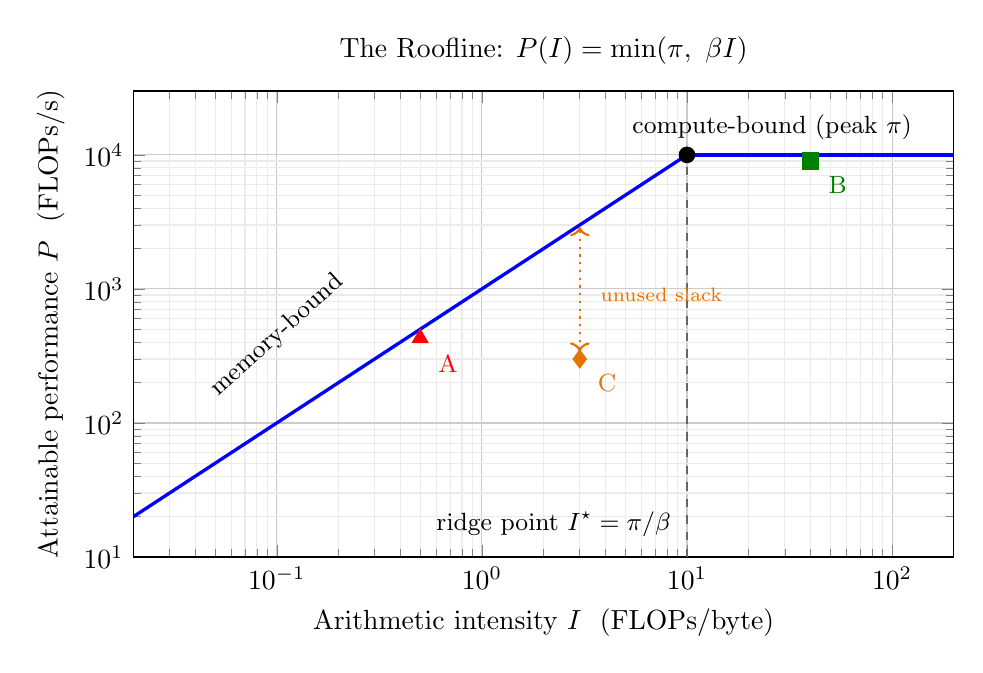
\begin{tikzpicture}
\begin{axis}[
    width=12cm, height=7.5cm,
    xmode=log, ymode=log,
    xlabel={Arithmetic intensity $I$ \ (FLOPs/byte)},
    ylabel={Attainable performance $P$ \ (FLOPs/s)},
    xmin=0.02, xmax=200, ymin=10, ymax=3e4,
    grid=both,
    major grid style={black!20},
    minor grid style={black!8},
    title={The Roofline: $P(I)=\min(\pi,\ \beta I)$},
]
% memory-bound slope (beta = 10^3) up to the ridge, then the flat compute roof (pi = 10^4)
\addplot[very thick, blue, domain=0.02:10, samples=2] {1000*x};
\addplot[very thick, blue, domain=10:200, samples=2] {10000};

% ridge point
\draw[dashed, black!60] (axis cs:10,10) -- (axis cs:10,10000);
\addplot[only marks, mark=*, mark size=2.8pt, black] coordinates {(10,10000)};
\node[anchor=south east, font=\small] at (axis cs:9.3,12) {ridge point $I^{\star}=\pi/\beta$};

% region labels
\node[font=\small, rotate=42] at (axis cs:0.1,450) {memory-bound};
\node[font=\small, anchor=south] at (axis cs:26,11000) {compute-bound (peak $\pi$)};

% three example kernels
\addplot[only marks, mark=triangle*, mark size=3.2pt, red] coordinates {(0.5,430)};
\node[anchor=north west, red, font=\small] at (axis cs:0.55,380) {A};
\addplot[only marks, mark=square*, mark size=3pt, green!50!black] coordinates {(40,9000)};
\node[anchor=north west, green!50!black, font=\small] at (axis cs:44,8200) {B};
\addplot[only marks, mark=diamond*, mark size=3.2pt, orange!90!black] coordinates {(3,300)};
\node[anchor=north west, orange!90!black, font=\small] at (axis cs:3.3,270) {C};
\draw[<->, dotted, orange!90!black, thick] (axis cs:3,340) -- (axis cs:3,2900);
\node[anchor=west, orange!90!black, font=\scriptsize] at (axis cs:3.4,900) {unused slack};
\end{axis}
\end{tikzpicture}
\par\smallskip
{\small Illustrative numbers: $\pi=10^{4}$, $\beta=10^{3}$, hence $I^{\star}=10$.
A is memory-bound (on the slanted roof), B is compute-bound (on the flat roof),
C sits below both and has room to improve.}
\end{center}

The story the roofline tells is diagnostic. For a given kernel one
computes (or profiles) its $I$ and its realised $P$. If the point
lies close to the slanted ceiling, the kernel is memory-bound;
further arithmetic optimisation is futile, and one should instead
pursue \emph{data reuse} (tiling, fusion, caching in shared memory).
If it lies close to the horizontal ceiling, the kernel is
compute-bound and one should instead pursue \emph{better
instructions} (tensor cores, lower precision, better algorithms).
If it lies below both ceilings, there is unexhausted slack, and
profiling is in order.

For accessible introductions to the roofline model, see the roofline
chapter of the JAX
\href{https://jax-ml.github.io/scaling-book/roofline}{\textit{Scaling
Book}} and the roofline entry of Modal's
\href{https://modal.com/gpu-glossary/perf/roofline-model}{\textit{GPU
Glossary}}.

\subsection{Multi-Level Rooflines}

In reality, a modern GPU does not have one bandwidth but many: HBM,
L2, L1/shared, and NVLink, each with its own $\beta$. One can
therefore draw multiple slanted ceilings, giving a laminated
roofline that distinguishes kernels limited by different levels of
the hierarchy. A kernel that fits comfortably in shared memory may
be compute-bound with respect to HBM but still memory-bound with
respect to its register file --- a useful distinction when deciding
where to spend one's optimisation effort.

\begin{aside}
One diagnostic subtlety: the arithmetic intensity of an operation
depends on what one chooses to count as ``transferred bytes.''
Counting traffic to HBM gives one curve; counting traffic between
shared memory and registers gives another; counting traffic across
the PCIe bus gives yet another. The roofline is a \emph{family} of
models, each answering a slightly different question. Know which
question you are asking.
\end{aside}

%%%%%%%%%%%%%%%%%%%%%%%%%%%%%%%%%%%%%%%%%%%%%%%%%%%%%%%%%%%%%%%%%%%%%%%%
\section{Asynchronous Execution, Streams, and CUDA Graphs}
%%%%%%%%%%%%%%%%%%%%%%%%%%%%%%%%%%%%%%%%%%%%%%%%%%%%%%%%%%%%%%%%%%%%%%%%

A feature that returns to haunt anyone who has ever tried to
benchmark GPU code is that, from the CPU's point of view, kernel
launches and most memory copies are \emph{asynchronous}. Issuing a
kernel enqueues it; the Python interpreter does not wait. This is a
feature, not a bug: it is precisely what allows a slow host language
to drive a fast accelerator.

\subsection{Serial and Concurrent Timelines}

Consider a pipeline consisting of a host-to-device copy (H2D), a
kernel, and a device-to-host copy (D2H). A strictly serial execution
waits for each to finish before beginning the next. (The timelines
below are modelled on those in NVIDIA's
\href{https://developer.nvidia.com/blog/how-overlap-data-transfers-cuda-cc/}{\textit{How
to Overlap Data Transfers in CUDA C/C++}}.)

\begin{center}
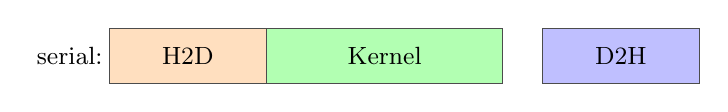
\begin{tikzpicture}[
    blk/.style={rectangle, draw=black!70, minimum height=0.7cm,
                font=\small, align=center},
]
\node[blk, fill=orange!25, minimum width=2cm] (h) at (0,   0) {H2D};
\node[blk, fill=green!30,  minimum width=3cm] (k) at (2.5, 0) {Kernel};
\node[blk, fill=blue!25,   minimum width=2cm] (d) at (5.5, 0) {D2H};
\node at (-1.5, 0) {\small serial:};
\end{tikzpicture}
\end{center}

With multiple streams and pinned memory, the copy engine and the
kernel engine can proceed in parallel, and a pipelined schedule
overlaps them:

\begin{center}
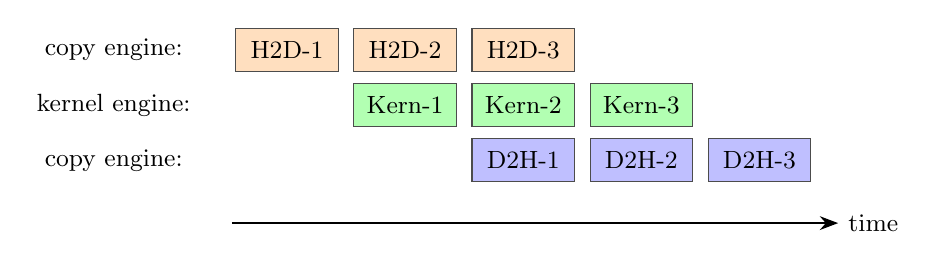
\begin{tikzpicture}[
    blk/.style={rectangle, draw=black!70, minimum height=0.55cm,
                font=\small, align=center},
]
\node at (-2.2, 1.3) {\small copy engine:};
\node at (-2.2, 0.6) {\small kernel engine:};
\node at (-2.2,-0.1) {\small copy engine:};

\node[blk, fill=orange!25, minimum width=1.3cm] at (0.0,  1.3) {H2D-1};
\node[blk, fill=orange!25, minimum width=1.3cm] at (1.5,  1.3) {H2D-2};
\node[blk, fill=orange!25, minimum width=1.3cm] at (3.0,  1.3) {H2D-3};

\node[blk, fill=green!30,  minimum width=1.3cm] at (1.5,  0.6) {Kern-1};
\node[blk, fill=green!30,  minimum width=1.3cm] at (3.0,  0.6) {Kern-2};
\node[blk, fill=green!30,  minimum width=1.3cm] at (4.5,  0.6) {Kern-3};

\node[blk, fill=blue!25,   minimum width=1.3cm] at (3.0, -0.1) {D2H-1};
\node[blk, fill=blue!25,   minimum width=1.3cm] at (4.5, -0.1) {D2H-2};
\node[blk, fill=blue!25,   minimum width=1.3cm] at (6.0, -0.1) {D2H-3};

\draw[-Stealth, thick] (-0.7,-0.9) -- (7, -0.9) node[right, font=\small] {time};
\end{tikzpicture}
\end{center}

\subsection{CUDA Graphs}

Each kernel launch incurs a non-trivial CPU-side cost. For a model
whose iteration consists of hundreds of small kernels, this launch
overhead can become a bottleneck in its own right. \textbf{CUDA
graphs} address this by allowing the programmer to \emph{capture} an
entire sequence of launches and their dependencies into a single
graph object, which the CPU then issues with one call.

\begin{center}
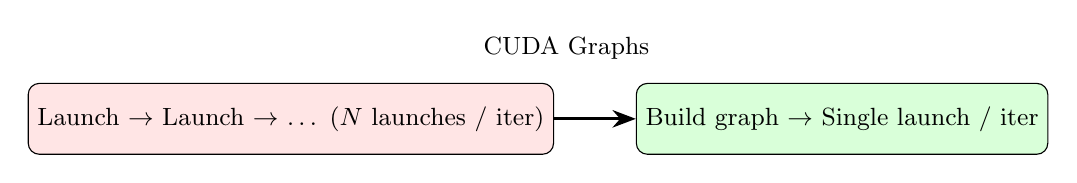
\begin{tikzpicture}[
    every node/.style={font=\small}
]
\node[rectangle, draw, rounded corners, fill=red!10,
      minimum width=4cm, minimum height=0.9cm] (a) at (0,0)
      {Launch $\to$ Launch $\to$ \dots \ ($N$ launches / iter)};
\node[rectangle, draw, rounded corners, fill=green!15,
      minimum width=4cm, minimum height=0.9cm] (b) at (7,0)
      {Build graph $\to$ Single launch / iter};
\draw[-Stealth, very thick] (a) -- (b);
\node at (3.5, 0.9) {CUDA Graphs};
\end{tikzpicture}
\end{center}

For inference workloads with static shapes, graph capture can yield
double-digit percentage speedups almost for free.

%%%%%%%%%%%%%%%%%%%%%%%%%%%%%%%%%%%%%%%%%%%%%%%%%%%%%%%%%%%%%%%%%%%%%%%%
\section{PyTorch Specifics and Practical Benchmarking}
%%%%%%%%%%%%%%%%%%%%%%%%%%%%%%%%%%%%%%%%%%%%%%%%%%%%%%%%%%%%%%%%%%%%%%%%

\subsection{Things PyTorch Does That Will Confuse You}

\begin{itemize}[leftmargin=1.5em, itemsep=3pt]
    \item \textbf{Kernels are asynchronous.} \texttt{time.time()}
          around a \texttt{forward} call measures \emph{launch time}
          on the CPU, not execution time on the GPU. To measure
          honestly, call \texttt{torch.cuda.synchronize()} before
          stopping the clock.
    \item \textbf{\texttt{tensor.item()} is a synchronisation
          point.} It forces a device-to-host copy, which stalls the
          CPU until the GPU has finished everything it is currently
          doing. Scattered \texttt{.item()} calls are a classic
          performance foot-gun.
    \item \textbf{Memory is cached, not freed.} PyTorch's caching
          allocator holds on to freed blocks rather than returning
          them to the OS, because \texttt{cudaMalloc}\slash
          \texttt{cudaFree} are expensive. Use
          \texttt{torch.cuda.memory\_allocated()} and
          \texttt{torch.cuda.memory\_reserved()} to tell the
          difference.
    \item \textbf{There is no single best kernel.}
          cuDNN ships a family of algorithms, and the best choice
          depends on shapes, strides, and hardware. Setting
\begin{quote}\small
          \texttt{torch.backends.cudnn.benchmark = True}
\end{quote}
          instructs cuDNN to benchmark candidates on the first
          encounter of each shape and cache the winner. For static
          shapes this is pure profit; for highly variable shapes it
          can be a net loss.
\end{itemize}

\begin{example}[The effect of \texttt{cudnn.benchmark}]
Consider a single \texttt{Conv2d} with $64$ filters of size
$3 \times 3$ applied to an input tensor of shape
$(32, 32, 64, 64)$. Measured kernel times, in nanoseconds:
\begin{center}
\renewcommand{\arraystretch}{1.2}
\begin{tabular}{@{}lrrc@{}}
\toprule
Setting & \texttt{benchmark=False} & \texttt{benchmark=True} & speed-up\\
\midrule
Forward (FP32)            & 1430 & 840  & $1.70\times$ \\
Forward+backward (FP32)   & 2870 & 2260 & $1.27\times$ \\
\bottomrule
\end{tabular}
\end{center}
A one-line change, a sizeable improvement.
\end{example}

\subsection{Measuring Performance Honestly}

Benchmarking is less glamorous than optimisation and twice as
important. The purpose is not to produce a single heroic number but
to identify \emph{where} a system is slow and \emph{by how much} a
candidate optimisation would help.

Use proper tools: \texttt{\%timeit} and \texttt{timeit.Timer} in
generic Python, and \texttt{torch.utils.benchmark} within PyTorch,
which handles warmup and synchronisation correctly and provides
statistics with error bars.

Guard against the usual pitfalls:
\begin{description}[leftmargin=1.5em, style=nextline]
    \item[Warmup.] The first few iterations pay for JIT compilation,
          kernel autotuning, and cache population. Throw them away.
    \item[Caching and preallocation.] A second run on the same
          tensors hits a hot cache. If cold performance is what
          matters, measure cold.
    \item[Randomisation.] Fixed inputs can accidentally take
          algorithmic fast paths. Randomise to make the benchmark
          representative.
    \item[Synchronisation.] On the GPU, call
          \texttt{torch.cuda.synchronize()} immediately before
          stopping the timer. Forgetting this is the most common
          source of suspiciously fast measurements.
\end{description}

\begin{remark}[Against premature optimisation]
Optimising a function that consumes two percent of runtime, even to
the point of eliminating it altogether, improves the program by at
most two percent. Profile first; optimise the dominant term;
iterate. This is a discipline more often praised than practised.
\end{remark}

\begin{remark}[The fallacy of GPU utilisation]
\texttt{nvidia-smi} cheerfully reporting $100\%$ GPU utilisation
does not mean the GPU is doing useful work. The utilisation counter
is true whenever any kernel is in flight, including tiny kernels
that move a few bytes around while the rest of the chip sits idle.
A better proxy is \emph{Model FLOPs Utilisation} (MFU): the ratio of
the FLOPs the model should perform per step to the peak FLOPs the
hardware could deliver in that time. MFU is also imperfect --- it
ignores memory traffic, among other sins --- but it is much harder
to fool.
\end{remark}
\end{document}